
\RequirePackage{cmap}

\documentclass[
    usenatbib,
]{mnras}

\usepackage[T1]{fontenc}
\usepackage[dvipsnames, x11names]{xcolor}

\renewcommand{\baselinestretch}{1.0} % Change to 1.65 for double spacing
\usepackage{showyourwork}
\usepackage{amsmath}
\usepackage{amsfonts}
\usepackage{amssymb}
\usepackage{mathrsfs}

\usepackage{xurl}
\urlstyle{tt}

\usepackage{booktabs}
\usepackage{graphicx}
\usepackage[
    % colorlinks=true, 
    % allcolors=blue,
]{hyperref}



\usepackage{libertine}
\usepackage[libertine]{newtxmath}
\usepackage[scaled=0.76]{beramono}
\usepackage{microtype}
\usepackage{csquotes}
\usepackage[capitalise]{cleveref}
%\usepackage{xspace}

\usepackage{standalone}
\usepackage{tikz}
\usetikzlibrary{
    calc,
    positioning,
    shapes,
}

\usepackage{siunitx}
\sisetup{
    range-units = single,
    range-phrase = {--},
    separate-uncertainty = true,
    multi-part-units = brackets,
    product-units = brackets,
    detect-weight = true,
    per-mode = symbol,
    mode = text,
}
\DeclareSIUnit\parsec{pc}
\DeclareSIUnit\au{au}
\DeclareSIUnit\mas{mas}

%REMOVE LATER
\usepackage{soul}

\usepackage{astro_bib_macro} %shortcuts of journals defined in this file

\newcommand{\todo}[1]{\textcolor{red}{[#1]}}
\newcommand{\timmy}[1]{\textcolor{red}{[\textbf{Timmy:} #1]}} % amazing

% Define macros
\newcommand{\IWA}{\ensuremath{\mathrm{IWA}}}
\newcommand{\hwo}{HabWorlds}

% Define the colors of the \rainbows
\definecolor{C0}{HTML}{ff0000}
\definecolor{C1}{HTML}{ff6d38}
\definecolor{C2}{HTML}{ecc86f}
\definecolor{C3}{HTML}{a4f89f}
\definecolor{C4}{HTML}{5af8c8}
\definecolor{C5}{HTML}{12c8e6}
\definecolor{C6}{HTML}{386df9}
\definecolor{C7}{HTML}{8000ff}

\newcommand{\rainbows}{%
    \textcolor{C0}{r}%
    \textcolor{C1}{a}%
    \textcolor{C2}{i}%
    \textcolor{C3}{n}%
    \textcolor{C4}{b}%
    \textcolor{C5}{o}%
    \textcolor{C6}{w}%
    \textcolor{C7}{s}%
    % \xspace
}

% Patch \hypertarget; for details, see 
% https://tex.stackexchange.com/a/17138/97669
\makeatletter
\newcommand{\affiliationtarget}[1]{\Hy@raisedlink{\hypertarget{#1}{}}}
\makeatother
\newcommand{\affiliationlink}[1]{\hyperlink{#1}{#1}}



% Chasing rainbows with the Habitable Worlds Observatory
\title{Chasing \rainbows{} with the Habitable Worlds Observatory}
%Scattering phase angle probed by directly imaged planets, or
%Don't ask us about contrast


% Authors are in alphabetical order:
\author[Sophia R. Vaughan et al.]{%
    Sophia R. Vaughan$^{\affiliationlink{1},}$\thanks{Correspondence:  \url{sophia.vaughan@physics.ox.ac.uk}}
    Kimberly Bott$^{\affiliationlink{2},\affiliationlink{28}}$,
    Sarah L. Casewell$^{\affiliationlink{3}}$,
    Nicolas B. Cowan$^{\affiliationlink{4}}$,
    David S. Doelman$^{\affiliationlink{5,19}}$,
    \newauthor 
    Timothy D. Gebhard$^{\affiliationlink{6},\affiliationlink{29}}$,
    Matthew Kenworthy$^{\affiliationlink{5}}$,
    Johan Mazoyer$^{\affiliationlink{7}}$,
    Maxwell A. Millar-Blanchaer$^{\affiliationlink{8}}$,
    \newauthor 
    Olivier Absil$^{16}$,
    Lisa Altinier$^{13}$,
    Pierre Baudoz$^{7}$,
    Ruslan Belikov$^{24}$,
    Alexis Bidot$^{9}$,
    Markus J. Bonse$^{29}$,
    \newauthor 
    Bernhard Brandl$^{5}$,
    Alexis Carlotti$^{9}$,
    Elodie Choquet$^{13}$,
    Niyati Desai$^{17}$,
    Kevin Fogarty$^{24}$,
    Jules Fowler$^{12}$,
    \newauthor
    Yann Gutierrez$^{7,14,22}$,
    Olivier Guyon$^{15,25,26,27}$,
    Sebastiaan Y. Haffert$^{15}$,
    Olivier Herscovici-Schiller$^{14}$, 
    \newauthor
    Adrien Hours$^{9}$,
    Roser Juanola-Parramon$^{20,21}$,
    Elina Kleisioti $^{5}$,
    Lorenzo König$^{16}$,
    Mariya Krasteva$^{23}$, 
    \newauthor
    Iva Laginja$^{7}$,
    Rico Landman$^{5}$,
    Lucie Leboulleux$^{9}$,
    David Mouillet$^{9}$,
    Mamadou N’Diaye$^{10}$,
    Emiel H. Por$^{18}$,
    \newauthor
    Laurent Pueyo$^{18}$,
    Frans Snik$^{5}$,
    Daphne M. Stam$^{30}$,
    Victor Trees$^{31,32}$,
    Dirk van Dam$^{5}$,
    Kyle van Gorkom$^{15}$,
    \newauthor
    Maaike van Kooten$^{11}$ 
    \newauthor \\%
    Affiliations are listed at the end of the paper
    % Timmy: I checked MNRAS and it seems that this is how they handle very long author lists. See, for example:
    % https://academic.oup.com/mnras/article/498/2/2354/5900562
    % I've also added some LaTeX magic to create links for the affiliations; if y'all agree that it's a good idea I can extend it to all authors?
}
\date{Draft version: \today}


\pagestyle{plain}
 
\begin{document} 

\maketitle

\begin{abstract}
NASA recently announced the Habitable Worlds Observatory (HWO), a coronagraphic mission to detect rocky planets in habitable zones, establish their habitability, and search for biosignatures. 
%Numerous instrumental and observational challenges have still to be overcome to design a coronagraphic mission with that goal. After a research phase aiming at the detection of a few tens of exo-Earth in the habitable zone, the Habitable Worlds Observatory will use its spectroscopic and polarimetric capabilities to probe these planets' atmosphere and surface properties. 
Surface liquid water is central to the definition of planetary habitability.
%
Photometric and polarimetric phase variations can show the presence of specularly reflecting oceans on exoplanets, in addition to being sensitive to rainbows and other cloud scattering effects. 
%
Direct imaging missions are optimised to detect planets near quadrature, which may obscure some of the phases at which these features are strongest. 
%
The range of scattering phases accessible for an exoplanet can be limited by its orbital inclination or the coronagraph's inner working angle. 
%
Planets that orbit close to edge-on have accessible phase angles limited by obscuration by the coronagraph. 
%
We use the list of target stars for the Habitable Worlds Observatory to estimate the number of exo-Earths that could be searched for non-Lambertian scattering phenomena. 
%
We find that exo-Earths in systems listed in this Habitable Worlds Observatory catalog will have a detectable Rayleigh scattering peak. 
%
The glint signature at planetary phase angles of 
%$\sim$50--70$^\circ$ 
$\sim$110--130$^\circ$ would be accessible to the Habitable Worlds Observatory in $\sim$14 systems, and the rainbow of water clouds at phases of 140--160$^\circ$ would be accessible in $\sim$42 systems, assuming a 62\,mas inner working angle (\IWA; 3$\lambda/D$ for a 6-m telescope at 600nm).
%
Increasing the \IWA to 2$\lambda/D$, increases the number of systems with detectable rainbows and glints by factors of roughly 2 and 3, respectively.
%
The number of systems in which an exo-Earth could be searched for these scattering phenomena increases with orbital eccentricity and scales approximately inversely with \IWA.     \end{abstract}

\begin{keywords}
planets and satellites: terrestrial planets -- 
instrumentation: high angular resolution -- 
planets and satellites: atmospheres
\end{keywords}

%%%%%%%%%%%%%%%%%%%%%%%%%%%%%%%%%%%%%%%%%%%%%%%%%%%%%%%%%%%%%%%%%%%%%%%%%%%%%%%%%

\section{Introduction}
\label{sec:intro}

%--------------------------------------------------------------------------------
\begin{figure*}%[t]
   \centering
   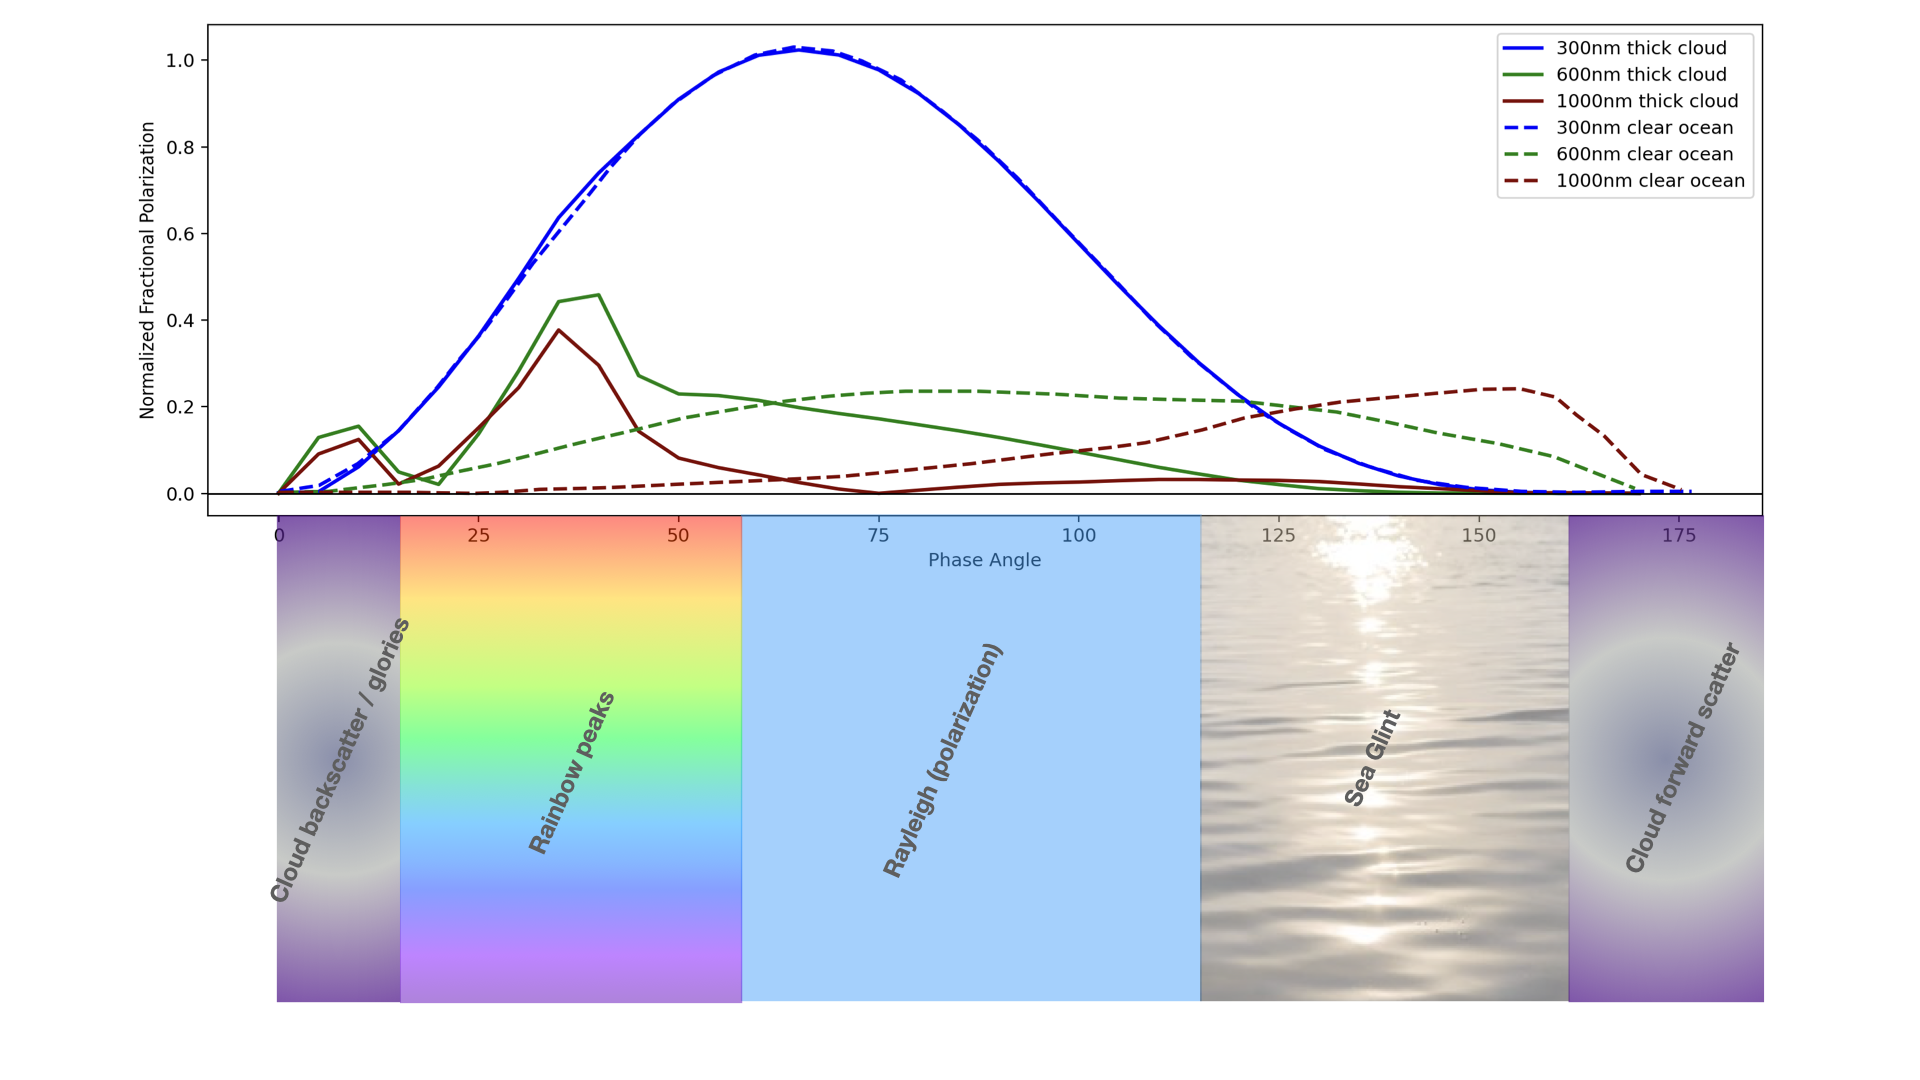
\includegraphics[width=\linewidth]{figures/Fig1IWAPol.png}
   \caption{BOTT PLOT this is a holder until Kim updates the figure}
    \label{fig:bottplot}
\end{figure*}
%--------------------------------------------------------------------------------

Signatures of habitability, from ocean glint to optical effects from condensates --- like the rainbow---should be some of the most distinct signals in an exoplanet's phase curve, particularly in polarized light.
%
However, depending on system architectures, some of these features can be obscured by the inner working angle of a coronagraph.

Surface liquid water is closely related to planetary habitability because it is essential for life as we know it.
%
To first order, the presence of liquid surface water can be predicted by the flux a planet receives from its star.
%
The habitable zone (HZ) describes the range of semi-major axes around a given main sequence star for which a rocky planet (or moon) may have the right temperature to maintain liquid surface water \citep{kasting93}. 
%
However, there are many factors that influence a planet's surface temperature and ability to hold liquid surface water, such as the atmospheric surface pressure and geological activity. 
%
Establishing the presence of liquid surface water on an exoplanet therefore provides important context for interpreting possible biosignatures.
%
Providing additional context to the habitability of an exoplanet is the presence of a water-cycle as evidenced by the characterization of a rainbow and other cloud optical effects. 

%The phase curves showing these features are distinct depending on the characteristics of the planet in both polarized and unpolarized measurements. Polarized and unpolarized phase curves and spectra each have their own strengths in characterization outlined below.


%%%%%%%%%%%%%%%%%%%%%%%%%%%%%%%%%%%%%%%%%%%%%%%%%%%%%%%%%%%%%%%%%%
\subsection{Exoplanet Phase Curves}

An exoplanet observed in an edge-on orbit will move through all phases and thus all scattering angles, while those viewed at higher inclinations will pass through a subset of these scattering angles.
%
If the planet is rotating, this supplies additional regular variations that can be used to place constraints on the heterogeneity of the planet and potentially map it.

The strengths of detailed phase curve analysis include mapping \citep{2001Natur.412..885F, berdyugina2019surface}, the detection of dark areas or glint indicative of seas \citep{groot2020, cowan2008inverting, lustig2019}, and the characterization of clouds through forward- and back-scatter, rainbows, and glories.
%
In polarized light an added potential benefit is the suppression of starlight from quiescent stars without explicitly requiring a coronagraph or starshade \citep{kemp1987}.

%%%%%%%%%%%%%%%%%%%%%%%%%%%%%%%%%%%%%%%%%%%%%%%%%%%%%%%%%%%%%%%%%%%

\subsection{Ocean Glint}

%As ocean glint is one of the few sources of specular reflection and is strongly polarized, it provides one of the best means to detect a signature of habitability in exoplanet phase curves. 
Ocean glint is from the specular (Fresnel) reflection of light off of smooth liquid surfaces at crescent phases.
%
In the total flux the signal of the glint will be most prominent at small planetary phase (large scattering) angles.
%
The maximum polarization occurs at the Brewster angle determined by the refractive indices at the interface; between air and liquid water this occurs at 53 degrees  \citep[a scattering angle of 127 degrees; see e.g. ][]{2008Icar..195..927W}.
%
It therefore varies slightly by wavelength and by sea and atmosphere composition.
%
In general on a planet the glint will be strongest in red wavelengths where the Rayleigh contribution to both the phase curve and attenuation are minimized \citep{Zugger_2011} and, conveniently, where the latitude-albedo effect (a degeneracy between polar brightness and glint) is also minimized \citep{2012ApJ...752L...3C}.
%
The strengthened glint signature at longer wavelengths has been observed in Earthshine measurements \citep{Emde2017,sterzik2019, takahashi2021}.
%
The broadening of the glint feature in the presence of wind-driven waves is well-described by the Cox-Munk solution \citep{CoxMunk1954}, shifts in both polarized and unpolarized light, and broadens across scattering angles in polarized light \citep{kopparla2018, Zugger_2010, treesandstam2019, trees2022}. 

The glint provides evidence of surface liquid bodies, which taken in the context of the temperature and condensates may be interpreted as the presence of liquid water.
%
The forward scattering from clouds can be confused with glint \citep{Robinson_2010} further motivating also probing the rainbow angle for context.
%
The cloud coverage fraction on ocean worlds can also be constrained with observations spanning the ultraviolet to near-infrared by the point phase curves at all wavelengths intersect in polarized light \citep{treesandstam2019}.
%
Additionally, \citet{trees2022} showed that glint can also be detected in spectropolarimetry while the planet is at phase angles placing it at the wide separations more easily probed with coronagraphs.
%how use to map, 
%seen in Earthshine
%strong signal for exoplanets
% disentangled from cloud coupled with rainbow
%disentangled from lattitude albedo coupled in polarization


%%%%%%%%%%%%%%%%%%%%%%%%%%%%%%%%%%%%%%%%%%%%%%%%%%%%%%%%%%%%%%%%%%%%

\subsection{Rainbows and Glories}

Rainbows, glories and other optical effects from condensates provide a wealth of information about an exoplanet \citep{karalidi2012rainbow, stam2008}.
%
In our own Solar System the polarized back scatter from Titan provided evidence that the world's reflectance was due to haze rather than a surface \citep{zellner1973polarization}, on Venus the rainbow and phase curve behavior with wavelength showed the clouds were $\sim$75\% H$_2$SO$_4$ -- water mixture also constraining the droplet size distribution \citep{hansenhovenier1974}, and the glory was later used to rule out some solutions for the unknown UV absorber \citep{petrova2018glory}.

In unpolarized light the forward scattering and backscatter from clouds can dramatically change the shape of a phase curve from Lambertian.
%
While the glory and rainbow are technically visible in any phase curve, their strongly polarized nature coupled with the suppression of signal from other effects at gibbous and full phases in polarized light make them far easier to characterize in polarized light (both in the degree of polarization and in full Stokes measurements) \citep{karalidi2011, stam2008, treesandstam2019}.
%
The rainbow angle depends on the refractive index and therefore varies with wavelength and depending on the species.
%
The feature being far more narrow than the glint allows more exact determination of the species.
%
The droplet size distribution also effects the shape of the rainbow and clouds of species in a solid phase can diverge from the Mie scattering that produces these features greatly, producing other optical effects particularly at narrow scattering angles \citep{bailey2007, hansentravis1974, Karalidi2012ice}.
%
In this paper we define our optimal angle for rainbow detection as the peak of the water droplet rainbow in visible wavelengths.
%
However, extending observations to angles closer to the star (smaller scattering angles, i.e.\ larger phase angles) would allow the full shape of the rainbow to be characterized and ensure the characterization of rainbows from other possible HZ condensates.
%
The glory is produced when the droplet radii much smaller than the wavelength of light and can allow further characterization as their angle, intensity, and shape also vary with the complex refractive index but primarily occur within 20 degrees scattering angle very close to full phase. 
%
%The glory (in the backscattering direction) and diffraction peak (in the forward scattering direction) are distinct features in the total reflected flux, but not in the degree of polarization. In principle, the degree of polarization goes to zero in the forward and backward scattering directions. See e.g. Fig. 1 of \citet{stam2008}, Fig. 5 of \citet{trees2022}, Fig. 3 of \citet{karalidi2011} and \citet{hansentravis1974}.}}

\subsection{Habitable Worlds Observatory}

The National Academy of Sciences Astronomy \& Astrophysics 2020 Decadal Survey \citep{decadal} recommended the first in a new \enquote{Great Observatories} program a telescope with the capability to detect signatures of habitability on about 25 habitable zone planets.
%
This assertion requires an instrument with a coronagraph capable of high contrast imaging at optical to near infrared wavelengths.
%
Following this release, NASA recently announced the start of the development of the Habitable Worlds Observatory (\hwo).
%
The precursor technology recommended by the Decadal Survey also lists ``direct imaging to probe polarized ocean glint on terrestrial planets'' as one of the priority capabilities \citep[Box E.1 in][]{decadal} for ground and space-based observatories.
%
The performance and precise characteristics of this telescope (on-axis or off-axis, exact diameter, type of segmentation, type of coronagraph) are still to be determined.
%
The development will be heavily influenced by the LUVOIR \citep{LUVOIR2019} and HabEx \citep{HabEx_2020} preparatory studies.
%
The Inner Working angle (\IWA) of the resulting telescope will depend on these choices, which in turn will have a significant impact on the expected exo-Earth yield \citep{Stark2019_exoplanetyield}.

The Extreme Coronagraph for Living Planetary Systems (ECLIPS) coronograph for LUVOIR was a proposed \SIrange{200}{2000}{\nano\meter} instrument for exoplanet characterisation, with a similar coronagraph operating between \num{450} and \SI{1800}{\nano\meter} planned for HabEx.
%
POLLUX, a proposed UV instrument for the LUVOIR study could also detect  polarised light from hot Jupiters at \SI{300}{\nano\meter} \citep{Bouret2018_pollux}.
%
However, because of the challenges associated with the design of a coronagraph in the UV, it appears to be unlikely that \hwo will include a UV high-contrast instrument sensitive to Earth-like planets.

%We ignore contrast in this study
%OWA -> should go in discussions

%\textbf{In this paper we...}
\subsection{Outline}

In this paper, we quantify the planetary phase angles that would be accessible for direct observations for hypothetical terrestrial planets orbiting in the habitable zones of HabWorlds target stars.
%
In \S 2.1, we describe the target list, in \S 2.2 we derive expressions for the range of phase angles given a few different limits, in \S 2.3, we describe Monte Carlo simulations to marginalize over the unknown orbital inclination and eccentricity of planets in these systems, and in \S 2.4, we outline how the planet/star contrast changes as a function of the planet's orbital phase.  
%
We present and discuss our results in \S 3 and conclude in \S 4. 
%the   the way that inclination and coronagraph inner working angle can limit the accessible phase angles  
% We minimally explore the contrast ratio as we are primarily exploring whether these scattering angles are reachable with inner working angle and outer working angle considered.

% We do not consider the particulars of specific planet scenarios as that work is completed by foward models

%We do not separate Stokes parameters as we are interested in where the net signal is achievable with IWA and OWA. 

%%%%%%%%%%%%%%%%%%%%%%%%%%%%%%%%%%%%%%%%%%%%%%%%%%%%%%%%%%%%%%%

%\section{Plots to Include}
%\label{sec:plots}
%\begin{enumerate}
%    \item \st{Cartoon defining various phase angles: orbital phase, scattering phase, $\beta$ ? (Sophia)}
%    \item Bott plot: annotated polarized and unpolarized phase curves for ocean world and cloudy worlds (Kim)
%    \item \st{3x3 cartoon showing effect of inclination and IWA compared to orbit (Sophia)}
%    \item Cumulative distribution functions, both simple (circular, edge-on), bit more realistic (circular, but range of inclinations), and full-on (range of inclinations and eccentricities). Max \& Matthew
%    \item Scatter plot of stellar effective temperature vs system distance (Timmy)
%\end{enumerate}
 
%%%%%%%%%%%%%%%%%%%%%%%%%%%%%%%%%%%%%%%%%%%%%%%%%%%%%%%%%%%%%%%%%%%%%%%%%%%%%%%%%%%%%%%%%%%%%%%%%%%%%%%%%%%%%%%%%%%%%%%%%%%%%%

%\section{Observing scattering phenomena}
\section{Methods}

%%%%%%%%%%%%%%%%%%%%%%%%%%%%%%%%%%%%%%%%%%%%%%%%%%%%%%%%%%%%%%%

\subsection{\hwo\ and Stellar Sample}
%\textcolor{blue}{Merge the 2 sections here into "Assumed technical specifications and sample"? I don't think this needs to be 2 subsections}
\hwo\ is still in the early stages of development, and the exact telescope and instrument design is as of yet undecided. 
%
In this work, we assume a \SI{6}{\meter} primary mirror, which is the currently favoured design for the observatory.
%
The observatory will utilise a coronagraph to suppress the stellar light and facilitate high-contrast observations of faint accompanying exoplanet. 
%
The \IWA{} of the coronagraph is currently undecided and will be driven by both the science requirements and technological limitations. 
%In this work, we investigate the scattering phase coverage obtainable for several choices for the \IWA\ of the observatory. 
%We also consider the Outer Working Angle (OWA) but for most targets this is not a limiting factor. 
%From the HabWorlds report. Inner Working Angle: The IWA defines the region near the star that cannot be accessed for direct imaging due to a coronagraphic mask, starshade obscuration, or an interferometric null. It depends on the architecture of the telescope, the starlight suppression system used, and the observation wavelength. While a nominal value could be defined by making assumptions about the design for Habitable Worlds Observatory, we choose instead to derive the IWA from the star list itself and Astro2020’s requirement that ~100 cumulative habitable zones be surveyed by direct imaging. As shown in the main table, an IWA near ~70 mas will be needed to access ~100 cumulative habitable zones, and would need to be achieved at all wavelengths of interest for spectral characterization. For any specific telescope and starlight suppression system architecture the IWA is typically proportional to wavelength; thus, the number of accessible HZs will strongly decrease as IWA(lambda) increases.
For ease of comparison, \cref{tab:IWA_OWA} lists the angular separations corresponding to multiples of $\lambda / D$ for a \SI{6}{\meter} telescope at representative visible and near infrared wavelengths of $\lambda = \SI{600}{\nano\meter}$ and $\SI{1}{\micro\meter}$.
 
\begin{table}
    \centering
    \caption{
        Conversion between $\lambda / D$ and \si{\mas} for different wavelengths, assuming $D = \SI{6}{\meter}$. 
        %\todo{We should use consistent wavelengths for this table, for the Bott Plot, and for the M\&M cumulative distribution function. Also update to use the only wavelength we choose.}
    }
    \label{tab:IWA_OWA}
    \begin{tabular}{ c c c c } 
    \toprule
     & $\lambda/D$ & mas (at \SI{600}{\nano\meter}) & mas (at \SI{1}{\micro\meter}) \\
    \midrule
    \midrule
    IWA & 1 & 20.63 & 34.38 \\
    IWA & 2 & 41.25 & 68.75 \\
    IWA & 3 & 61.88 & 103.13 \\
    IWA & 4 & 82.51 & 137.51 \\
    \midrule
    OWA & 32 &  660.05 & 1100.08 \\
    OWA & 64 & 1320.09 & 2200.16 \\
    \bottomrule
    \end{tabular}
\end{table}


\hwo\ is currently envisioned to observe the stars stated in the NASA Exoplanet Exploration Program's Mission Star List for the Habitable Worlds Observatory.
%
\footnote{\url{https://exoplanets.nasa.gov/internal_resources/2645_NASA_ExEP_Target_List_HWO_Documentation_2023.pdf}}
%
This list comprises $\sim$160 stars, the majority of which are Sun-like dwarfs; 66~F~dwarfs, 55~G~dwarfs, 40~K~dwarfs, and 3~M~dwarfs.
%
The target list is constructed assuming a maximum planet magnitude of $R_c = 31$ and a contrast floor of \num{2.5e-11}. 
%with an occurrence rate of rocky planets in the optimistic habitable zone to be $\eta_{\oplus}$ = 0.24 \citep{decadal}. 
The corresponding adopted habitable zone limits are a semi-major axis of \SIrange{0.95}{1.67}{\au} for a solar twin, planet sizes between \SIrange{0.8}{1.4}{} Earth radii, and for non-solar stars, scale as square root of the bolometric luminosity normalized to the Sun. 
%
This range of orbital separation corresponds to the \enquote{conservative habitable zone} \citep{kasting93, kopparapu13}. 
%
The authors of the report determined that these are the nearby stars (maximum distance \SI{25}{\parsec}) for which exo-Earths would be the most observable for an imaging survey of habitable zones with a \SI{6}{\meter} telescope. 

In what follows, we consider hypothetical Earth-size planets orbiting at the right distance from each star to receive the same flux as the Earth receives from the Sun.
%
By construction, such planets should be observable at quadrature phase by HabWorlds. 

%%%%%%%%%%%%%%%%%%%%%%%%%%%%%%%%%%%%%%%%%%%%%%%%%%%%%%%%%%%%%%%

\subsection{Maximum scattering phase angle coverage}
\label{sec:Delta_phi}

The coronagraph can obscure part of the planet's orbit which, as demonstrated in \cref{fig:annotated-orbit}, can prevent the planet from being observed at high and low scattering angles. 
%
The range of scattering phase angles that can be observed will depend on the \IWA{} of the coronagraph as well as the shape and orientation of the exoplanet's orbit.

\begin{figure}
    \centering
    \includestandalone{tikz/annotated-orbit}
    \caption{
        An illustration of an edge-on circular orbit showing that the coronagraph can obscure the exoplanet at high and low scattering phase angles.
        %
        This can prevent observations of scattering phenomena which could be used to indicate the habitability and atmospheric composition of the exoplanet. 
        %\timmy{Maybe mention that this is a simplified illustration with a circular orbit, plus we are basically looking at an edge-on system?}
    }
    \label{fig:annotated-orbit}
\end{figure}

%%%%%%%%%%%%%%%%%%%%%%%%%%%%%%%%%%%%%%%%%%%%%%%%%%%%%%%%%%%%%%%

\subsubsection{Circular edge-on orbits}


In the non-eccentric case (i.e., with a circular orbit and where the coronagraphic mask centred on the star), minimum ($\varphi_\mathrm{min}$) and maximum ($\varphi_\mathrm{max}$) scattering phase angles accessible are symmetric about 90 degrees. 
%
We define the angle $\Delta \varphi$ such that: 
\begin{equation}
 \label{eq:Delta_phi}
    \Delta \varphi 
    = \varphi_\mathrm{max} - \varphi_\mathrm{min}
    =  2(\varphi_\mathrm{max} - 90^\circ) 
    =  2(90^\circ-\varphi_\mathrm{min} ) 
\end{equation}
% \begin{equation}
%     \label{eq:Delta_phi}
%     \Delta \varphi 
%     = \varphi_\mathrm{max} - \varphi_\mathrm{min}
%     =  2(\varphi_\mathrm{max} - 90) 
%     =  2(\varphi_\mathrm{min} + 90)
% \end{equation}

% {\color{Green} Victor Trees: Do you mean:
%INDEED, THERE MUST HAVE BEEN A TYPO, THX!
% %
% \begin{equation}
%     \Delta \varphi 
%     = \varphi_\mathrm{max} - \varphi_\mathrm{min}
%     =  2(\varphi_\mathrm{max} - 90^\circ) 
%     =  2(90^\circ-\varphi_\mathrm{min} ) \notag
% \end{equation}
%
% } 

The on-sky projected planet distance, $r_\mathrm{proj}$ (in \si{\au}) is shown in \cref{fig:scattering-angle} assuming a non-eccentric circular orbit with a semi-major $a$ (in \si{\au}) at a distance $d_*$ (in \si{\parsec}) from the observer. 
%
The scattering phase angle $\varphi$ in this set up follows the equation,
\begin{equation}
    \sin(\varphi) = \frac{r_\mathrm{proj}}{a}
\end{equation}
%
Using small angles, $r_\mathrm{proj} = \delta d_*$ where $\delta$ is the angular separation on-sky.
%
We access the minimum scattering angle when the projected distance reaches the inner working angle separation $\delta = \mathrm{IWA}$. 
%
Using \cref{eq:Delta_phi}, we deduce:
%
\begin{equation}
    \label{eq:scattering_angle}
    \cos\left(\dfrac{\Delta \varphi}{2}\right) = \frac{\mathrm{IWA \cdot d_*}}{a}
\end{equation}
 %
\begin{figure}
    \centering
    \includestandalone{tikz/scattering-angle}
    \caption{
        The on-sky projected planet distance, $r_\mathrm{proj}$, of a planet with a semi-major $a$ at a distance $d_*$.
        %
        The on-sky angular separation as viewed by the observer is $\delta$.
        %
        The scattering phase angle, $\varphi$, is the angle between the line of sight to the star and the line connecting the star and planet.  
    }
    \label{fig:scattering-angle}
\end{figure}

\Cref{fig:scatterplot} shows $\Delta \varphi$ for the systems in the \hwo\ target list, assuming an IWA of \SI{62}{\mas} ($3 \lambda / D$ coronagraph at $\SI{600}{\nano\meter}$). 
\timmy{60 (as in the abstract), or 62?}
%
%This assumes each planet has a semi-major axis such that it receives an Earth-equivalent instellation, which is provided in the input star list.
%
For edge-on circular orbits, it will be possible to observe Rayleigh scattering for all targets and rainbows will be accessible in some cases.

\begin{figure*}
    \centering
    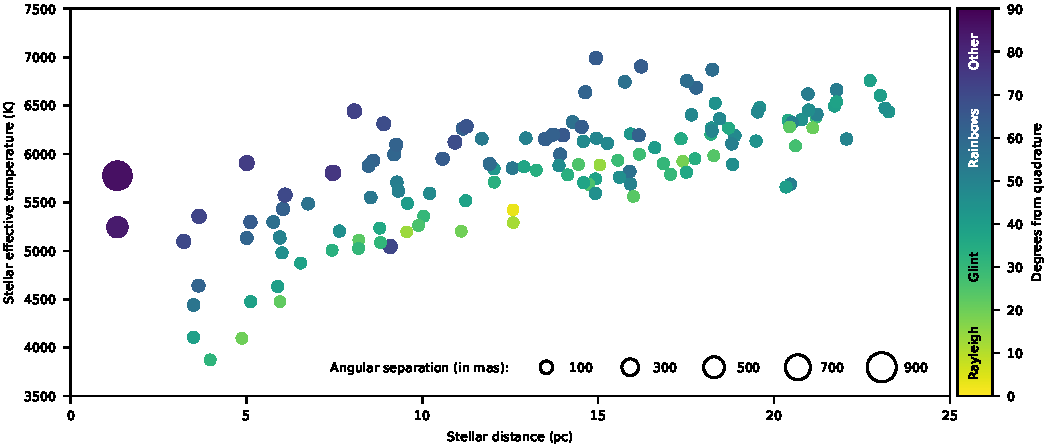
\includegraphics{figures/scatterplot.pdf}
    \caption{
        Scatter plot for the target sample, showing stellar effective temperature and stellar distance.
        %
        The size of the points represents the angular separation of the star and planet in milliarcseconds as presented in the target list.
        %
        The colour of the points shows $\Delta \varphi$ assuming a circular edge-on orbit at a semi-major axis corresponding to an Earth-like instellation for an IWA of 62 mas.
        %
        Additionally, the colour bar indicates the atmospheric phenomenon that can be detected where phenomena from the bottom of the colour bar up to the indicated colour are detectable for that system.
        %
        Thus, dark blue points are systems which have the most key features, as systems in which the angles required to see the rainbow are probed will also have the angles required to see the Rayleigh scattering probed.
    }
    \label{fig:scatterplot}
    \script{create-scatterplot.py}
\end{figure*}

%%%%%%%%%%%%%%%%%%%%%%%%%%%%%%%%%%%%%%%%%%%%%%%%%%%%%%%%%%%%%%%

\subsubsection{Circular inclined orbits}

Most systems will not be viewed as edge on from Earth.
%
For a given system with inclination $i$, we have identified 2 regimes, which are shown in \cref{fig:orb-grid}:

\begin{enumerate}
    \item If the inclination is relatively face-on, then the coronagraph mask does not obscure any part of the sky-projected orbit, and the maximum scattering phase angle coverage depends solely on the disk inclination ;
    \item When parts of the orbit  are hidden by the focal plane mask, the scattering phase angle coverage only depends on the \IWA{} and orbital semi-major axis. 
\end{enumerate}

\begin{figure}%[htb]
   \centering
   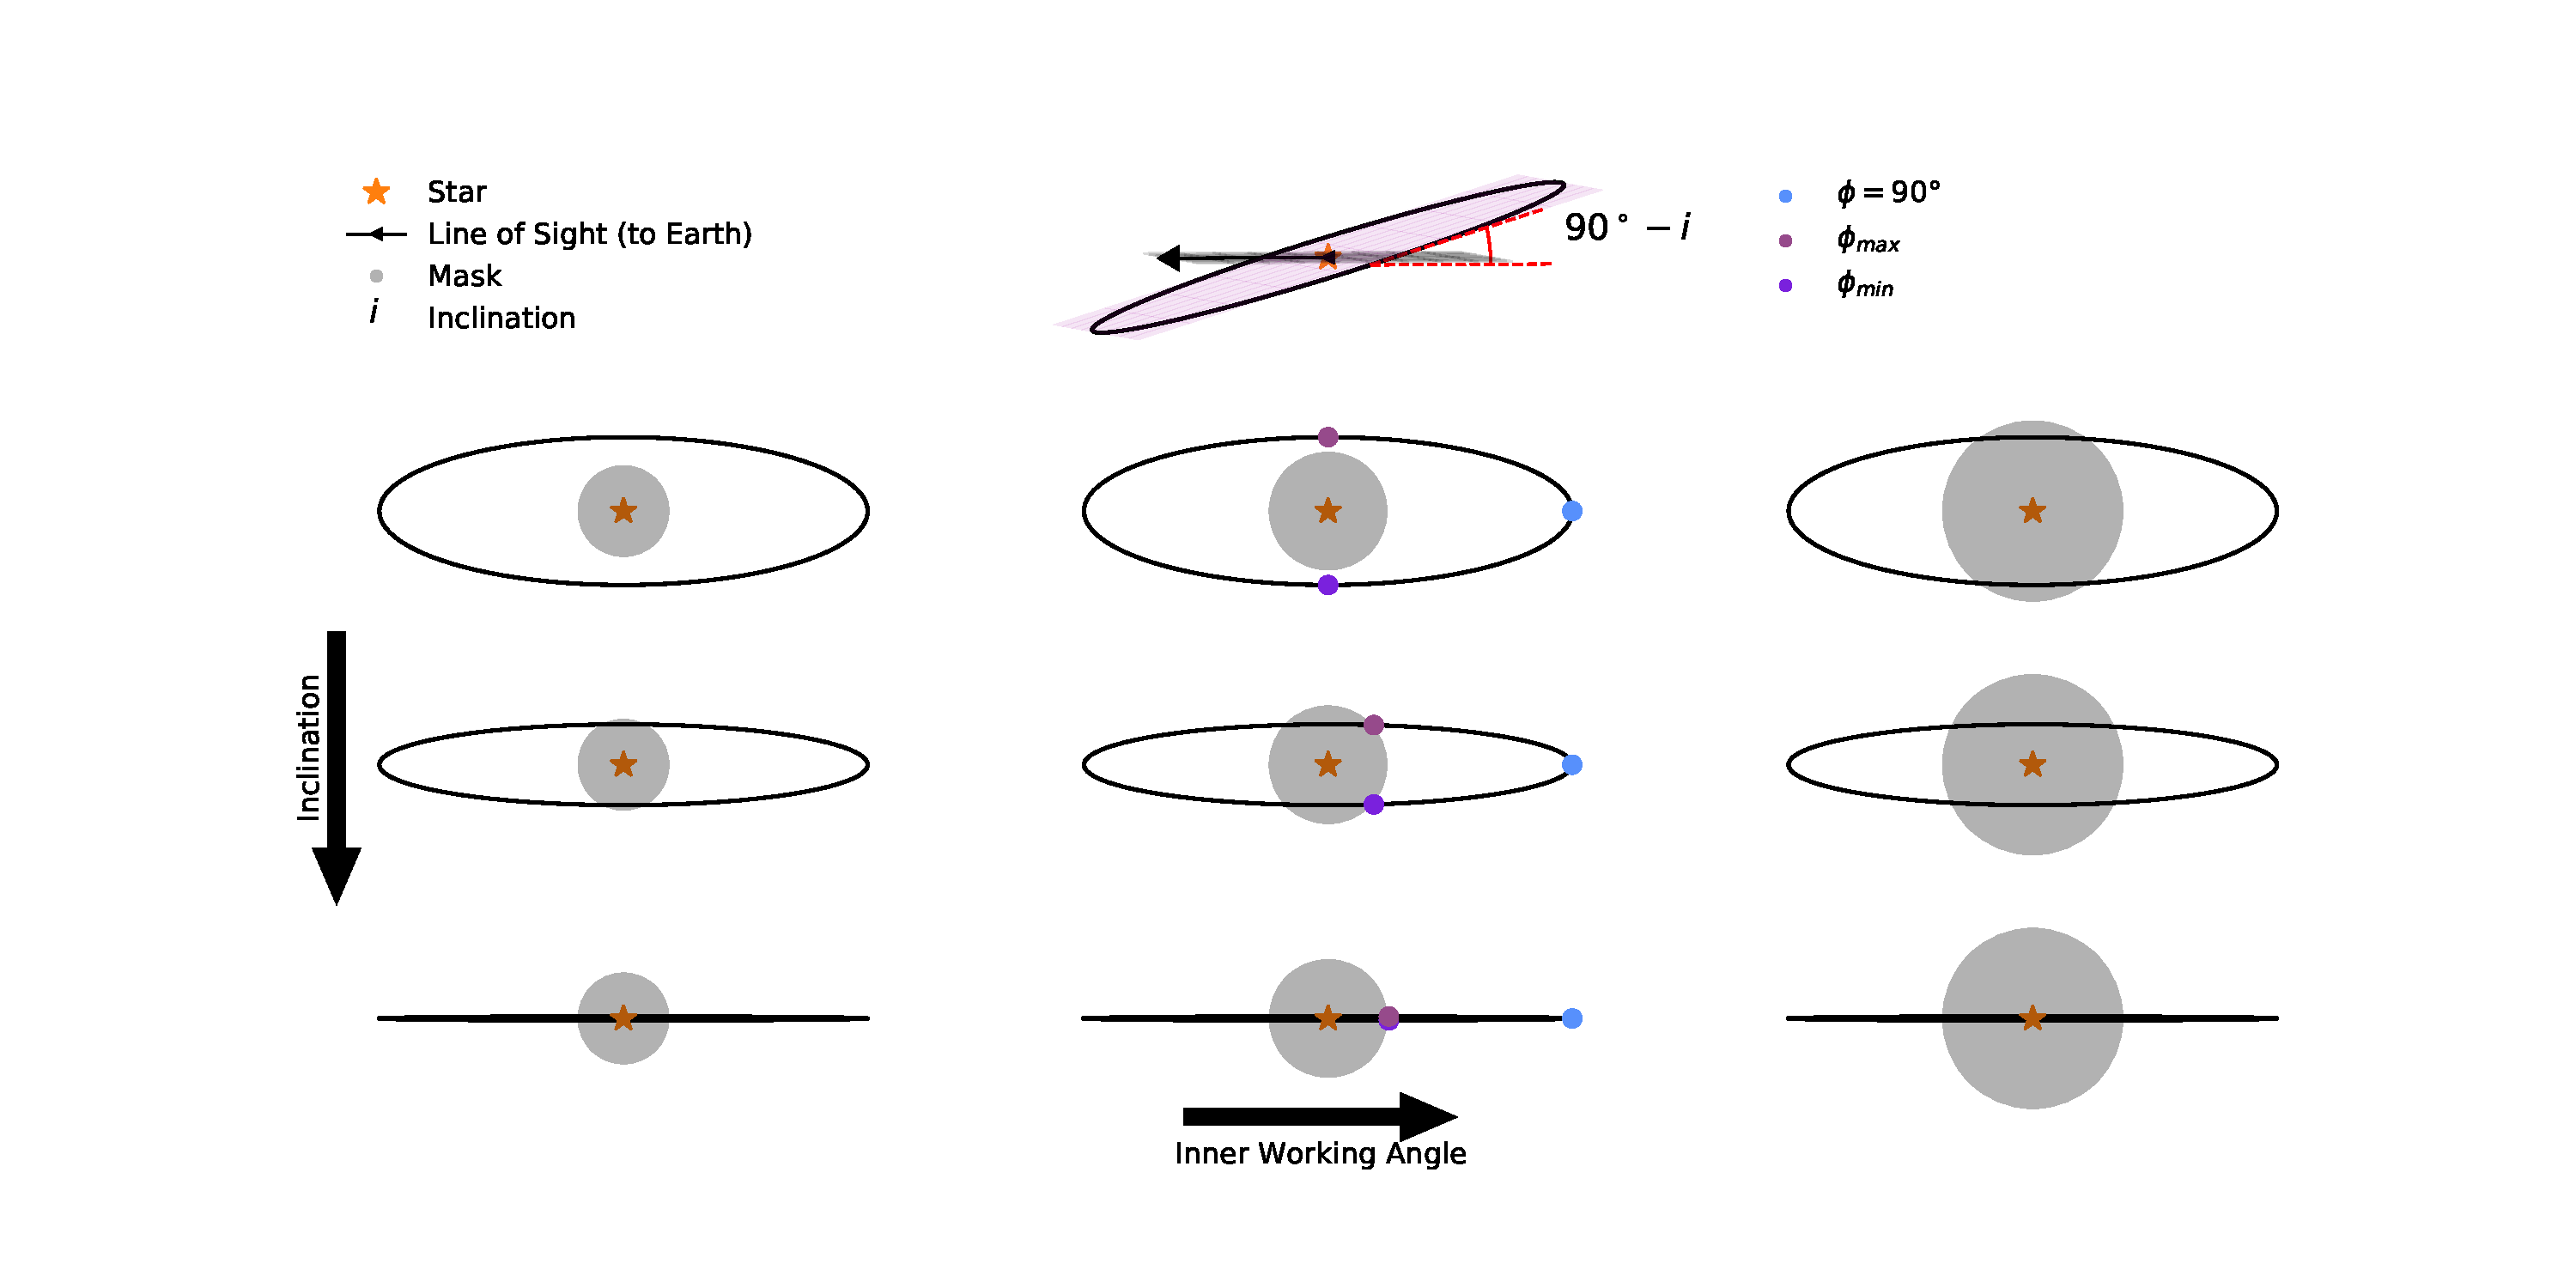
\includegraphics[width=0.99\columnwidth]{figures/orb-grid.pdf}
   \caption{
        The scattering phase angles accessible to a direct imaging mission can be limited by orbital inclination or by the coronagraphic inner working angle.
        %
        If the orbital inclination is close to face-on (top panels) then the scattering phase angles probed throughout an orbit are limited by inclination; for circular orbits accessible scattering phases are $\phi \in 90^\circ \pm i$. 
        %
        For orbital inclinations close to edge-on (bottom panels) the planet goes through all phases, but the scattering phase angles near 0$^\circ$ and 180$^\circ$ are not accessible due to obscuration by the coronagraph mask; for circular orbits, the accessible scattering phases are $\phi \in 90^\circ \pm \arcsin({\rm IWA}\cdot d_*/a)$.
    }
    \label{fig:orb-grid}
    \script{plot-orb-grid.py}
\end{figure}

Using \cref{eq:scattering_angle}, we deduce the equation for inclined circular orbits: 
\begin{equation}
\label{eq:Delta_phi_max}
    \Delta \varphi = 
    \begin{cases}
        2 i & \textrm{for} \cos(i) > \frac{\mathrm{IWA}\; d_* }{a}
  \\ 
        2  \cos^{-1}\left(\dfrac{\mathrm{IWA}\cdot d_* }{a}\right)  & \textrm{for} \cos(i) < \frac{\mathrm{IWA}\; d_* }{a}
    \end{cases}\,.
\end{equation}

%%%%%%%%%%%%%%%%%%%%%%%%%%%%%%%%%%%%%%%%%%%%%%%%%%%%%%%%%%%%%%%

%\subsubsection{Eccentric orbits}


%The inclination $i$ is sampled such that $\cos(i)$ follows a uniform distribution, $\cos(i) \sim \mathcal{U}(0, 1)$.

%%%%%%%%%%%%%%%%%%%%%%%%%%%%%%%%%%%%%%%%%%%%%%%%%%%%%%%%%%%%%%%
\subsection{Monte Carlo Simulations}

\subsubsection{Circular randomly inclined orbits}
\label{sec:circular}

For each star on the \hwo\ target list, we generate $1000$  hypothetical habitable planets at the Earth-equivalent-flux semi-major axis. 
%
The orbital inclinations are randomly drawn from a distribution uniform in $\cos i$. 
%
We then use \cref{eq:Delta_phi_max} to determine the range of accessible scattering phase angles for each hypothetical planet.
%
The solid lines in \cref{fig:betaallofit} show the cumulative distribution of the maximum and minimum accessible scattering phase angles normalised to the total number of systems in \hwo\ target list, depending on the choice of inner working angle.  

%%%%%%%%%%%%%%%%%%%%%%%%%%%%%%%%%%%%%%%%%%%%%%%%%%%%%%%%%%%%%%%

\begin{figure*}[t]
    \centering
    \includegraphics[width=0.95\textwidth]{figures/accessible_phase_angles.png}  
    \caption{
        \todo{shouldn't lambda/D for 600nm give 21, 41, 62, 83 mas?} 
        Cumulative distributions of the most extreme scattering phase angle accessible for different \IWA where the solid lines are for randomly inclined circular orbits and the dashed lines are for randomly orientated elliptical orbits.
        %
        The top x axis indicates the minimum scattering phase angle and the bottom x axis indicates the maximum.
        %
        These are symmetric about quadrature (90 degrees) \todo{is this true for elliptical orbits?}.
        %
        The y axis indicates the number of systems divided by the number of Monte Carlo samples and is thus normalised to the number of systems in the target list.
        %
        The secondary y axis indicates the number of systems assuming only 24 percent of them contain an Earth-like exoplanet in the habitable zone.
    }
    \label{fig:betaallofit}
    \script{plot_n_versus_phase.py}
\end{figure*}

\subsubsection{Eccentric randomly inclined orbits}
\label{sec:eccentric}
We repeat the Monte Carlo simulation from \cref{sec:circular} assuming the orbital eccentricity follows a beta distribution with shape parameters $a=0.867$ and $b=3.03$ \citep{2013MNRAS.434L..51K}. 
%
We randomly drew 1000 random orbits for each star and determined the sky-projected orbits following, e.g., \cite{2010exop.book...15M}. Eccentricities were drawn from the beta distribution, and inclinations were uniform in $\cos i$. \Cref{fig:ball-o-yarn} shows a sample of the generated orbits with the filtered \IWA's
%
%Each plot has been scaled such that the habitable zone occupies the same radius, hence the \IWA's vary in apparent size compared to the orbit.
%
We then calculated the minimum and maximum accessible scattering phase angles for of \IWA's of 21, 42, 63 and 84 mas which correspond to 1, 2, 3 and 4 times $\lambda / D$ at $\SI{600}{\nano\meter}$.
%
The dashed lines in \cref{fig:betaallofit} shows the normalised cumulative distribution of the accessible angles for each of the \IWA, when accounting for orbital eccentricity.
%
We also calculate which targets would be observable at the scattering phase angles where ocean glint, rainbows, or the Rayleigh peak occur.
%
The cumulative distribution over \IWA\ of the number of systems, normalised to the total number of systems, where each scattering phenomena is visible is shown in \cref{fig:accessible_phase_angles}.
%
 
\subsection{Simulating contrast curves}
\todo{Kim and David: is this done?}

A second parameter that is crucial for detecting features like rainbows and ocean glint on Earth-like planets is the contrast, that is, the relative flux of the reflected light from the planet divided by the stellar flux. 
%
While this is not the main focus of this paper, it is important to consider that the contrast and polarised contrast are not constant as a function of scattering phase angles.
%
This is due to a combination of the changing illumination fraction of the exoplanets Earth facing surface and scattering effects.
%
Here, we aim to present some simplified examples of the impact of the scattering angle dependent contrast on the detectability of rainbow and glint features. 
%
We note that these calculations are by no means complete or exact, given the many variables that go into modelling reflected fluxes and polarization fractions of an Earth-like planet \citep{ treesandstam2019,trees2022}.


The NASA Exoplanet Exploration Program’s Mission Star List for the Habitable Worlds Observatory includes an estimated contrast ratio for an Earth twin in the habitable zone for every star. 
%
The contrast is calculated as 
\begin{equation}
C = F_p/F_* = p \phi (\alpha) (R_p/a)^2,
\end{equation}
where $p$ is the geometric albedo, $\phi (\alpha)$ is the integral phase function at phase angle $(\alpha)$, $R_p$ is the planet’s radius, and $a$ is the separation of the planet from its star. 
%
The assumptions that went into these calculations are that the orbits are circular, the geometric albedo is $p=0.2$, and that the scattering phase function, $\phi(\alpha)$, can be described by a simple Lambertian reflectance phase function, for example, isotropic scattering.
%
These calculations give a good order-of-magnitude calculation for the contrast of Earth-like planets around nearby stars.
%
Therefore, in this work, we will assume that the calculated contrasts given in the list correspond to the reflected flux at quadrature and normalize the scattering phase functions to this point.
%
We note that we do not aim to accurately calculate the absolute scaling of the contrast, as this depends on many factors and would have required some of the work for the star list to be redone.

We use the scattering phase functions from \cite{treesandstam2019} for an Earth-like planet with an ocean surface with patchy clouds and a wind-speed of $\SI{7}{\meter\per\second}$ at $\SI{670}{\nano\meter}$.
%
The $\SI{670}{\nano\meter}$ is close to the centre of the Rc band for Vega ($\SI{642}{\nano\meter}$). 
%
We normalize the reflected light curve at the value of 90 degrees (quadrature) and multiply it with the contrast.
%
In addition, we map the orbital phase for circular orbits to the scattering phase angle and the on-sky separation given an inclination of $90$ degrees.
%
Together, they give the reflected light contrast as a function of separation for a full orbit.
%
We multiply this flux with the degree of polarisation and retrieve the polarised contrast.
%
The resulting contrast curves are shown in \cref{fig:contrasts} for three of the closest target stars, the G~dwarf $\alpha$~Cen~A, the K~dwarf $\epsilon$~Eri and the M~dwarf Lalande~21185.

\begin{figure*}%[t]
   \centering
   \includegraphics[width=0.99\textwidth]{figures/Contrast_vs_separation_inclination_angle_90.pdf}
   \caption{
    The reflected light contrast and orbital separation of an Earth-like planet with an ocean surface and patchy clouds over a planetary orbit assuming an orbital inclination of $90^\circ$ for the stars $\alpha$ Cen A, $\epsilon$ Eri and Lalande 21185.
    %
    The solid line indicates the contrast in unpolarised light with the contrast at quadrature marked by a solid dot.
    %
    The polarised component is indicated by the colored dots for which the color represents the scattering phase angle from quadrature.
    %
    The light grey points show the quadrature contrasts of the other targets in the star list and the dashed lines indicate $1,2$ and $3$ times the \IWA\ for \hwo.
    }
    \label{fig:contrasts}
    \script{plot_contrasts.py}
\end{figure*}

%%%%%%%%%%%%%%%%%%%%%%%%%%%%%%%%%%%%%%%%%%%%%%%%%%%%%%%%%%%%%%%%%%%%%%%%%%%%%%%%%%%%%%%%%%%%%%%%%%%%%%%%%%%%%%%%%%%%%%%%%%%%%%

\section{Results}

%\todo{Is there a plot for this? How many systems could we see? Why is it different to non-eccentric cases?}
%\timmy{No plot / results yet; see above.}
%\todo{Sophia: what is features\_plot\_peak.png showing?}
%\timmy{Good question --- maybe Matt or Max know how the data for this was generated? Matt: yes, it's all in showyourwork right now. I ran 1000 sims for each target with a random eccentric orbit, then pulled out the betamax and betamin angles for each of the 1000 realisations. Max's plots encode the completeness as a function of phase angle, showing that you get about 10 percent more phenomena. }

%%%%%%%%%%%%%%%%%%%%%%%%%%%%%%%%%%%%%%%%%%%%%%%%%%%%%%%%%%%%%%%

\subsection{The effect of eccentricity}
\label{sec:result_eccentricity}
As shown in \cref{fig:betaallofit}, allowing the planet's orbit to be eccentric can have a noticeable affect on the number of systems that can be observed at each scattering phase angle.
%
This is because, Kepler's second law ensures that eccentric planets spend more time at orbital separations greater than their semi-major axis, and hence are more likely to peak out from behind the coronagraph \IWA{} and extreme orbital phases (albeit with worse contrast due to the greater star--planet separation).
%
The eccentricity does not significantly effect the number of systems for smaller inner working angles as the systems in \hwo{} target list where chosen based on their on-sky separation quadrature and therefore the shape of the orbit has little affect for \IWA{} smaller than cut used in the selection. It is, however, important to account for orbital eccentricity when the \IWA{} of the coronoagraph is larger than the \IWA{} used to filter the target list otherwise the number of systems observable at extreme phase angles would be under predicted.

%%%%%%%%%%%%%%%%%%%%%%%%%%%%%%%%%%%%%%%%%%%%%%%%%%%%%%%%%%%%%%%

\subsection{Observable scattering phenomenon}
\label{sec:results_scattering_phenomena}

In this section we consider the number of stars around which different scattering phenomena could be observable for different \IWA{}.
%
We first define the phase angles over which various these phenomena are accessible, in Table~\ref{tab:phase_ranges}.
%
We note that these ranges should all be considered approximate, as the exact phase angles where these effects are dominant depend on the details of the atmospheric and surface properties, as well as the wavelengths being observed.
%
Nonetheless, this exercise can provide valuable insights on the effects of \IWA{} choice. 

\cref{fig:accessible_phase_angles} shows the number of systems in which key scattering phenomena will be observable for different \IWA{}.
%
The \IWA{} of \hwo's coronagraph will depend on the primary mirror diameter, observing wavelength and how well a coronagraph of a given size can suppress the glare of the host star.
%
The smaller the \IWA{}, the more features we will be observable and in more systems. 

\begin{table}
    \centering
    \caption{
        The ranges of phase angles for the different scattering phenomena considered here.
    }
    \label{tab:phase_ranges}
    \begin{tabular}{ c c c c } 
    \toprule
     & $\varphi_{min}$ & $\varphi_{peak}$ & $\varphi_{max}$ \\
    \midrule
    \midrule
    Rainbows & 22 & 42 & 63 \\
    Rayleigh & 50 & 70 & 110 \\
    Ocean Glint & 130 & 150 & 170 \\
    Glory & 0 & 5 & 10 \\
    \bottomrule
    \end{tabular}
\end{table}


    % features = {r'Rainbow': (127,138,158),
    %         r"Rayleigh": (90,110,130),
    %         r"Ocean Glint": (50,30,10),
    %         r"Glory": (10,5,0),
    %         }


The Rayleigh scattering feature appears near quadrature and is therefore observable in the most systems.
%
This feature is caused by atmospheric gases and can therefore be used to determine if a planet has an atmosphere.
%
The rainbow feature appears further from quadrature but will still be observable in a significant fraction of systems.
%
This feature will only be present if the atmosphere contains spherical droplets, potentially indicating the presence of liquid water.
%
The position and shape of the peak is sensitive to the properties of the droplets allowing their nature to be determined if the peak of the rainbow feature can be reached.
%
The ocean glint feature occurs even further from quadrature and so is observable in fewer systems. In most systems, only the first half of the feature is observable but this can still be used to identify a liquid ocean on the surface of the planet.
%
A key indicator of habitability. Finally, it is possible to view the glory scattering feature in one system, Alpha Cen A.
%
\todo{maybe we want a table of some numbers in this section}

\begin{table}
    \centering
    \caption{
        Number of stars around which the peak phase angle of each phenomena is detectable, expressed in $mas$ and $\lambda/D$ for $\lambda=600$nm. 
    }
    \label{tab:nstars_detect}
    \begin{tabular}{ c c c c } 
    \toprule
      & \multicolumn{3}{c}{IWA}
    \\
     & 21$mas$ & 41$mas$ & 62$mas$
    \\
     & $2\lambda/D$ & $3\lambda/D$ & $4\lambda/D$ 
    \\
    \midrule
    \midrule
    Rainbows & 90 & 42 & 18 \\
    Rayleigh & 152 & 115 & 65 \\
    Ocean Glint & 43 & 14 & 5 \\
    % Glory & 0 & 5 & 10 \\
    \bottomrule
    \end{tabular}
\end{table}

%%%%%%%%%%%%%%%%%%%%%%%%%%%%%%%%%%%%%%%%%%%%%%%%%%%%%%%%%%%%%%%

\subsection{Contrast Curves}
\label{sec:results_contrast}

The accessible scattering phase angles is not the factor that needs to be considered when determining what scattering features are observable.
%
The contrast of the planet is also an important factor to consider.
%
\cref{fig:contrasts} shows approximate contrast curves for three of the stars in the \hwo\ target list assuming edge-on orbits.
%
The over all contrast varies significantly for each system and throughout the orbit.
%
The observability of these planets will depend on the star light suppression of the coronagraph which is influenced by its \IWA{}.
%
It is not possible to predict how much the state of the art of coronagraphy will have advanced by the time \hwo{} is built.
%
However, when its design is being finalised, it will be important to consider both the accessible scattering phase angles and contrast limits when deciding on the \IWA{} of the coronagraph, if these features are to be observed.

%%%%%%%%%%%%%%%%%%%%%%%%%%%%%%%%%%%%%%%%%%%%%%%%%%%%%%%%%%%%%%%

%\subsection{The glory of Alpha Cen}%Halelujah
%\label{sec:ealpha-cen}
%\textbf{Glory science, what it tells us (Kim)}
% Kim will write para on science of glory (what tells us, vaguely why appears here) 

%%%%%%%%%%%%%%%%%%%%%%%%%%%%%%%%%%%%%%%%%%%%%%%%%%%%%%%%%%%%%%%

\begin{figure*}
    \centering
    \includegraphics{figures/ball_of_yarn.pdf}  
    \caption{
        %Are we putting all of these somewhere?  Its prob about 7 pages worth in total?
        Random examples of the eccentric orbits generated for the stellar sample.
        %
        The orbits are scaled by the Earth-equivalent flux distance. 
        %
        The concentric circles marked by the dashed lines indicate inner working angles of 20.6, 41.3, 61.9, and \SI{82.5}{\mas}, corresponding to 1, 2, 3, and 4\,$\lambda / D$ respectively (assuming $\lambda = \SI{600}{\nano\meter}$ and $D = \SI{6}{\meter}$).
        %
        The figure illustrates that the \IWA\ can significantly affect the range of scattering phases observable with each orbit.
    }
    \label{fig:ball-o-yarn}
    \script{make_yarn_plot.py} % most awesome command in this paper.  This knitter approves.
\end{figure*}
 
%\begin{figure*}
%    \centering
%    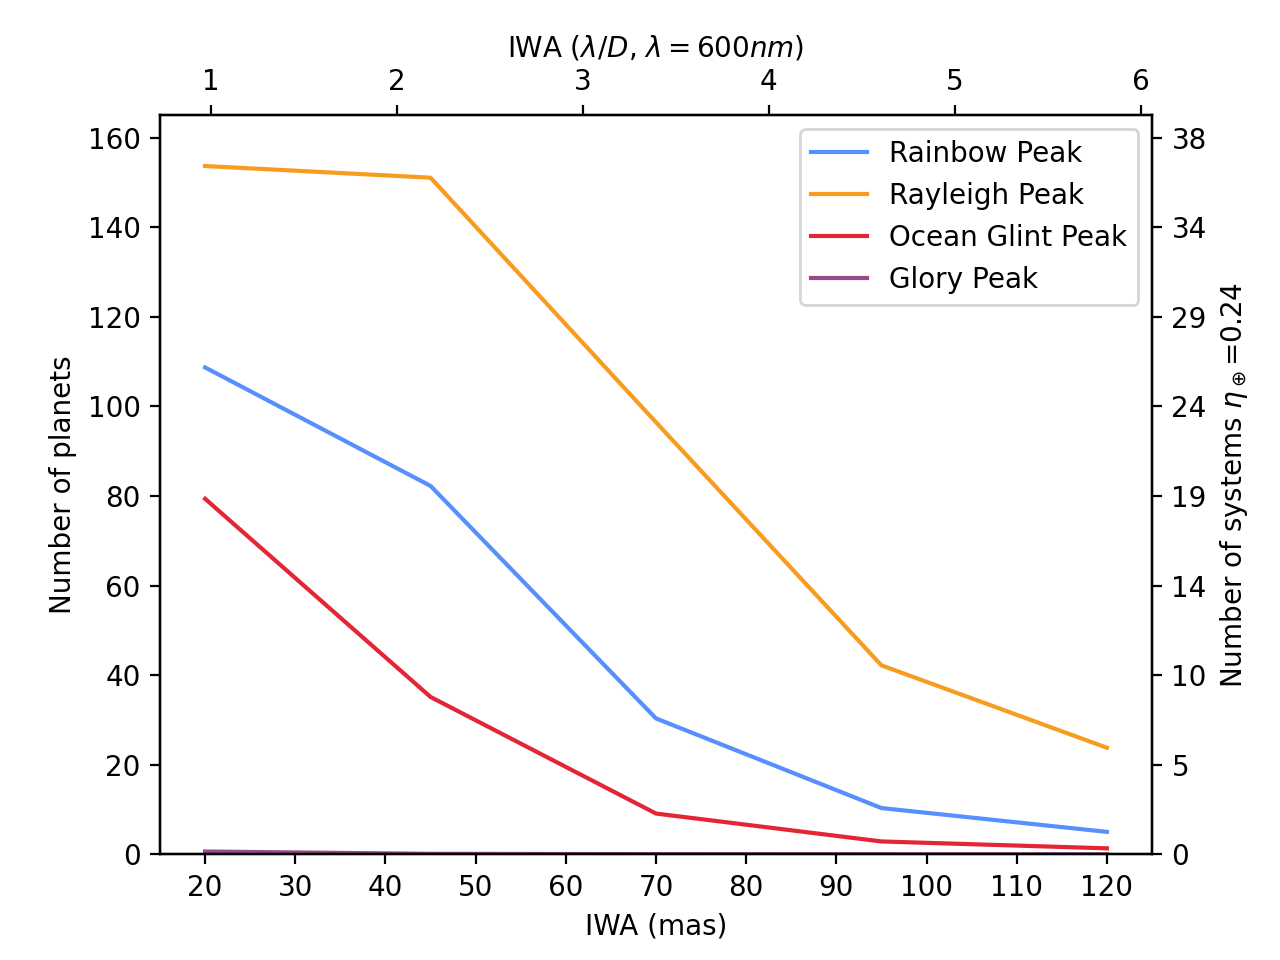
\includegraphics[width=0.6\textwidth]{figures/features_plot_peak.png}  
%    \caption{
%        Number of systems vs inner working angle
%    }
%    \label{fig:accessible_phase_angles}
%\end{figure*}

\begin{figure*}
    \centering
    \includegraphics[width=0.95\textwidth]{figures/nplanets_vs_iwa.png}  
    \caption{
        The number of systems for which key scattering features (Rayleigh scattering, rainbows, ocean glint and glories) can be observed as a function of \IWA{}.
        %
        Each subplot contains three lines where the dashed line shows the number of systems where the start of the scattering feature can be observed, the solid line shows the number of systems that reach the peak of the feature and the dot-dashed line the number where the scattering angles of the end of the feature are observable.
        %
        The bottom $x$ axis gives the \IWA{} of the coronograph in milliarcseconds which is converted to $\lambda/D$ for $\lambda=\SI{600}{\nano\meter}$ and $D=\SI{6}{\meter}$ for the top $x$ axis.
        %
        The secondary $y$ axis indicates the number of systems that each feature would be observable in assuming only 24\% of them contain an Earth-like exoplanet in the habitable zone.
        %
        It is worth noting that the Glory feature is only observable in one system, Alpha Cen A. 
    }
    \label{fig:accessible_phase_angles}
    \script{plot_features_vs_iwa.py}
\end{figure*}



%\subsection{Contrast Curves}
%\label{sec:contrast}

%%%%%%%%%%%%%%%%%%%%%%%%%%%%%%%%%%%%%%%%%%%%%%%%%%%%%%%%%%%%%%%%%%%%%%%%%%%%%%%%%%%%%%%%%%%%%%%%%%%%%%%%%%%%%%%%%%%%%%%%%%%%%%

\section{Conclusions}
%What did we determine? 
%Can we actually detect this stuff for anything in this sample? 
%Do we need to not something about things like A stars which are not included in the sample - they were rejected by the list creators - do we need to comment on this?  - we decided nope.

The Habitable Worlds Observatory is a coronagraphic space mission envisioned to detect and characterise Earth-like exoplanets in the 2040's. 
%
The instrument design and capabilities are still under development and thus can be driven by the science goals of the mission.
%
In this work, we investigated the possibility of using \hwo{} to detect scattering phenomena on terrestrial exoplanets, including ocean glint, which could establish a planet's habitability. 

We primarily focused on the range of scattering phase angles and therefore which scattering phenomena could potentially be observed given the limitation of the coronagraphic \IWA{}.
%
Coronagraphy is a rapidly advancing field, and it is hard to predict what the capabilities of \hwo{} will be.
%
Assuming a \SI{60}{\mas} \IWA{}, all 160 systems in the NASA Exoplanet Exploration Program's Mission Star List for the Habitable Worlds Observatory would be observable at scattering phases with Rayleigh features, but the rainbows of water clouds would only be accessible in $\sim$55 systems, and ocean glint in $\sim$20 systems.
%
The habitability of Earth analogs in the remaining 140 systems would have to be established by less direct means like rotational mapping to identify continents and oceans \citep[e.g.,][]{2009ApJ...700..915C,lustig2019}.   
%

The number of habitable zones that can be probed by \hwo{} increases with decreasing \IWA{}. 
%
The desire to detect and characterize a large number of Earth-like exoplanets, and the intrinsic frequency of such planets, will drive the choice of coronagraphic \IWA{} for this mission.
%
We have shown that only $\sim$10\% of Earth-like exoplanets imaged with \hwo{} could be imaged at a sufficiently wide range of phase angles to establish the presence of surface liquid water via its specular reflection.  
%
The habitability of remaining targets would have to be established by less direct means.
%
While we briefly considered the contrast ratio of the scattering features, we did not investigate the feasibility of detecting them given their contrast. 
%
This will be an important task once the instrument design and capabilities are better defined and could drive the design of the coronagraph. 

\section*{Software/Data Availability}

The NASA ExEP target list containing the data used for these simulations is available online.
%
\footnote{\url{https://exoplanets.nasa.gov/exep/science-overview/}}
This work has made use of \textsf{numpy}
 \citep{NumPy2020}, \textsf{scipy} \citep{scipy_2020}, \textsf{matplotlib} \citep{matplotlib2007}, and \textsf{astropy},\footnote{\url{https://www.astropy.org}} a community-developed core Python package and an ecosystem of tools and resources for astronomy \citep{astropy:2013, astropy:2018, astropy:2022}.

\section*{Acknowledgements}

The workshop on which this manuscript is based was made possible thanks to the logistical and financial support of the Lorentz Center, Leiden, Netherlands.
%
This workshop was supported by NOVA  and by the European Research Council (ERC) under the European Union's Horizon 2020 research and innovation programme (grant agreement n°866001 - EXACT).
%
This research has made use of NASA's Astrophysics Data System Bibliographic Services and the SIMBAD database, operated at CDS, Strasbourg, France. 
%
SRV acknowledges funding from the European Research Council (ERC) under the European Union’s Horizon 2020 research and innovation program under grant agreement No 805445.
%
SLC acknowledges support from an STFC Ernest Rutherford Fellowship. 
%
TDG acknowledges funding from the Max Planck ETH Center for Learning Systems.
%
Specific grant funding and any other specific requirements
%
KMB acknowledges support from NASA Habitable
%
Worlds grant No. 80NSSC20K152, and previous support for related work supported by NASA Astrobiology Institute's Virtual Planetary Laboratory under Cooperative Agreement Number NNA13AA93A.

% Add references
\bibliographystyle{mnras}
\bibliography{bib}


\section*{Author affiliations}
\begingroup
% \footnotesize
\itshape
\affiliationtarget{1}{$^{1}$} Department of Astrophysics, University of Oxford, Denys Wilkinson Building, Keble Road, Oxford OX1 3RH, UK\\
\affiliationtarget{2}{$^{2}$} Department of Earth and Planetary Sciences, University of California, Riverside, CA 92521, USA \\
\affiliationtarget{3}{$^{3}$} Centre for Exoplanet Research, School of Physics and Astronomy, University of Leicester, University Road, Leicester, LE1 7RH, UK\\
\affiliationtarget{4}{$^{4}$} Department of Earth \& Planetary Sciences and Department of Physics, McGill University, 3600 rue University, Montréal, QC, H3A 2T8, Canada\\
\affiliationtarget{5}{$^{5}$} Leiden Observatory, Leiden University, P.O. Box 9513, 2300 RA Leiden, The Netherlands\\
\affiliationtarget{6}{$^{6}$} Max Planck Institute for Intelligent Systems, Max-Planck-Ring 4, 72076 Tübingen, Germany \\
$^{7}$ LESIA, Observatoire de Paris, Université PSL, CNRS, Sorbonne Université, Université de Paris, F-92195 Meudon, France \\
$^{8}$ Department of Physics, University of California, Santa Barbara, CA 93106, USA \\
$^{9}$ Université Grenoble Alpes, CNRS, IPAG, 38000 Grenoble, France \\
$^{10}$ Université Côte d'Azur, Observatoire de la Côte d'Azur, CNRS, Laboratoire Lagrange, France \\
$^{11}$ National Research Council Canada, Herzberg Astronomy and Astrophysics Research Center, Victoria, B.C. Canada \\
$^{12}$ University of California, Santa Cruz, USA  \\
$^{13}$ Aix Marseille Univ, CNRS, CNES, LAM, Marseille, France \\
$^{14}$ DTIS, ONERA, Université Paris Saclay, 91123 Palaiseau, France \\
$^{15}$ Steward Observatory, University of Arizona, 933 North Cherry Avenue, Tucson, Arizona \\
$^{16}$ STAR Institute, Université de Li\`ege, All\'ee du Six Ao\^ut 19c, 4000 Li\`ege, Belgium \\
$^{17}$ Department of Astronomy, California Institute of Technology, Pasadena, CA, 91125, USA \\
$^{18}$ Space Telescope Science Institute, 3700 San Martin Drive, Baltimore, MD 21218, USA \\
$^{19}$ SRON Netherlands Institute for Space Research, Niels Bohrweg 4, 2333 CA, Leiden, The Netherlands \\
$^{20}$ NASA Goddard Space Flight Center, 8800 Greenbelt Rd, Greenbelt, MD  20771, USA \\
$^{21}$ University of Maryland Baltimore County, 1000 Hilltop Cir, Baltimore, MD 21250, USA \\
$^{22}$ DOTA, ONERA, 92322 Châtillon, France \\
$^{23}$ European Space Agency, ESTEC, Keplerlaan 1, 2200 AG Noordwijk, The Netherlands \\
$^{24}$ NASA Ames Research Center, Bldg. 245, Moffett Field, USA \\
$^{25}$ Subaru Telescope, NAOJ, USA \\
$^{26}$ College of Optical Sciences, University of Arizona, Tucson, AZ 87521, USA \\
$^{27}$ Astrobiology Center, 2 Chome-21-1, Osawa, Mitaka, Tokyo, 181-8588, Japan \\
\affiliationtarget{28}{$^{28}$} NASA Nexus for Exoplanet System Science, Virtual Planetary Laboratory Team, Seattle, WA 98195, USA \\
\affiliationtarget{29}{$^{29}$} ETH Zurich, Institute for Particle Physics \& Astrophysics, Wolfgang-Pauli-Str. 27, 8092 Zurich, Switzerland \\
\affiliationtarget{30}{$^{30}$} Delft University of Technology, Kluyverweg 1, 2629 HS Delft, The Netherlands \\
\affiliationtarget{32}{$^{31}$} Department of Geoscience \& Remote Sensing, Delft University of Technology, Stevinweg 1, 2628 CN, Delft, the Netherlands \\
\affiliationtarget{31}{$^{32}$} Royal Netherlands Meteorological Institute (KNMI), Utrechtseweg 297, 3731 GA, de Bilt, The Netherlands \\
\endgroup


\end{document} 

